\documentclass[11pt,sigconf]{acmart}

\usepackage{booktabs} % For formal tables

\graphicspath{{figure/}{figures/}}

% Copyright
%\setcopyright{none}
%\setcopyright{acmcopyright}
%\setcopyright{acmlicensed}
\setcopyright{rightsretained}
%\setcopyright{usgov}
%\setcopyright{usgovmixed}
%\setcopyright{cagov}
%\setcopyright{cagovmixed}


% DOI
\acmDOI{10.475/123_4}

% ISBN
\acmISBN{123-4567-24-567/08/06}

%Conference
\acmConference[CSCI-5502 '21]{CSCI-5502 Data Mining Summer 2021}{June 2021}{Boulder, CO, USA} 
\acmYear{2021}
\copyrightyear{2021}

\acmPrice{15.00}


\begin{document}
\title{CSCI 5502 Project Proposal}
\titlenote{This proposal is part 2 of the CSCI-5502 Data Mining Project}
\subtitle{Global Risk Perception During the COVID-19 Pandemic}

\author{Son Pham}
\authornote{Note}
\orcid{1234-5678-9012}
\affiliation{%
  \institution{CU Boulder}
  \streetaddress{Address}
  \city{Boulder} 
  \state{Colorado} 
  \postcode{80309}
}
\email{son.pham-2@colorado.edu}

\author{Kyle Rogers}
\orcid{1234-5678-9012}
\affiliation{%
  \institution{CU Boulder}
  \streetaddress{Address}
  \city{Boulder} 
  \state{Colorado} 
  \postcode{80309}
}
\email{kyro3301@colorado.edu}

\author{Firstname Lastname}
\orcid{1234-5678-9012}
\affiliation{%
  \institution{CU Boulder}
  \streetaddress{Address}
  \city{Boulder} 
  \state{Colorado} 
  \postcode{80309}
}
\email{email@domain.com}

\author{Firstname Lastname}
\orcid{1234-5678-9012}
\affiliation{%
  \institution{CU Boulder}
  \streetaddress{Address}
  \city{Boulder} 
  \state{Colorado} 
  \postcode{80309}
}
\email{email@domain.com}


% The default list of authors is too long for headers}
\renewcommand{\shortauthors}{S. Pham et al.}


\begin{abstract}
This paper focuses on how COVID-19 information was communicated within and between different countries, reactions of governments to the pandemic, and attitudes and risk perceptions people had towards the virus. The major questions to answer are how digital communications influenced people’s interpretation of the news, what their responses to the new laws and mandates were, and their beliefs and concerns about it versus other world issues.\footnote{This is an abstract footnote}
\end{abstract}

%
% The code below should be generated by the tool at
% http://dl.acm.org/ccs.cfm
% Please copy and paste the code instead of the example below. 
%
\begin{CCSXML}
<ccs2012>
   <concept>
       <concept_id>10002951.10003317.10003359.10011699</concept_id>
       <concept_desc>Information systems~Presentation of retrieval results</concept_desc>
       <concept_significance>500</concept_significance>
       </concept>
   <concept>
       <concept_id>10002978.10003029.10003032</concept_id>
       <concept_desc>Security and privacy~Social aspects of security and privacy</concept_desc>
       <concept_significance>300</concept_significance>
       </concept>
   <concept>
       <concept_id>10002950.10003648</concept_id>
       <concept_desc>Mathematics of computing~Probability and statistics</concept_desc>
       <concept_significance>300</concept_significance>
       </concept>
   <concept>
       <concept_id>10002951.10002952</concept_id>
       <concept_desc>Information systems~Data management systems</concept_desc>
       <concept_significance>500</concept_significance>
       </concept>
   <concept>
       <concept_id>10002951.10002952.10003219</concept_id>
       <concept_desc>Information systems~Information integration</concept_desc>
       <concept_significance>500</concept_significance>
       </concept>
   <concept>
       <concept_id>10002951.10002952.10002953</concept_id>
       <concept_desc>Information systems~Database design and models</concept_desc>
       <concept_significance>500</concept_significance>
       </concept>
   <concept>
       <concept_id>10002951.10002952.10003197</concept_id>
       <concept_desc>Information systems~Query languages</concept_desc>
       <concept_significance>500</concept_significance>
       </concept>
 </ccs2012>
\end{CCSXML}

\ccsdesc[500]{Information systems~Presentation of retrieval results}
\ccsdesc[300]{Security and privacy~Social aspects of security and privacy}
\ccsdesc[300]{Mathematics of computing~Probability and statistics}
\ccsdesc[500]{Information systems~Data management systems}
\ccsdesc[500]{Information systems~Information integration}
\ccsdesc[500]{Information systems~Database design and models}
\ccsdesc[500]{Information systems~Query languages}

% We no longer use \terms command
%\terms{Theory}

\keywords{Data Mining, Covid-19, Risk Perception, Communication}


\maketitle


\section{Introduction}

This is the introduction to the introduction section, introducing the problem statement and motivation behind the chosen project. What knowledge and how would you apply that knowledge? What is interesting that you hope to find?

\subsection{Motivation}

Go in detail about the problem statement and motivation.

Lorem ipsum dolor sit amet, consectetur adipiscing elit.
Sed aliquam nisl turpis, sit amet mollis leo accumsan vel.
Donec semper turpis dui, a porttitor lorem tincidunt id.
Phasellus gravida, purus non faucibus euismod, lectus tortor maximus elit, vestibulum lobortis purus turpis non urna.
Fusce feugiat lectus ut massa molestie, non interdum augue porta.
Nunc dapibus odio nec neque cursus, ut lacinia velit rutrum.
Duis tempor nulla velit, sed pellentesque nunc imperdiet ut.
Phasellus eget hendrerit neque.
Suspendisse aliquet nulla id sem aliquam aliquam sed a orci.
Duis sem est, hendrerit nec porttitor sit amet, maximus sed nulla.
Suspendisse et dictum massa.
Morbi non diam nec orci sodales eleifend.
Etiam eget finibus purus, a malesuada ipsum.
Nullam ac nisi nec elit faucibus aliquet.
Nulla feugiat velit sed sodales eleifend.
Donec orci nulla, viverra et mi in, sagittis egestas urna.

\begin{figure}[htbp]
  \centering
  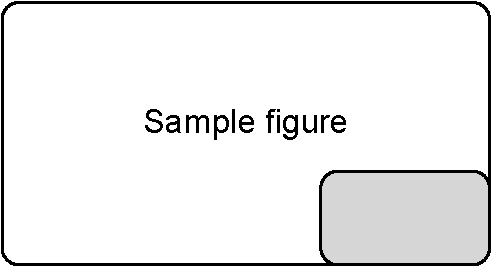
\includegraphics[scale=0.5]{figure1}
  \caption{Sample figure}
  \label{fig:sample}
\end{figure}

\subsubsection{Subsubsection if needed}

Integer eleifend quam et odio iaculis, at elementum augue aliquam.
Ut eu nibh nec urna finibus semper fermentum id purus.
Aliquam eu sollicitudin libero.
Cras viverra elit congue erat pulvinar, vitae vehicula tortor interdum.
Aliquam commodo mi sapien, ullamcorper egestas velit tempor nec.
Quisque sapien velit, fringilla non vulputate nec, lacinia in dui.
Nam vestibulum volutpat ante, eu sodales enim tincidunt vel.



\section{Literature Survey}

Describe and site all any literature found.

\subsection{Literature subsection (if needed)}

Go in detail about each literature



\section{Proposed Work}

What do you need to do for data collection, preprocessing (cleaning, integrating, transforming, etc.) processing for derived data, design, evaluation...
Describe how it is different that what has been done previously from your literature survey (or if replicating).

\subsection{Proposed Work subsection (if needed)}

Go in detail about each proposed work



\section{Data Set}

Make sure you have the data set!. Provude URL and details about the data set (similar to hw1, ch2, etc)

\subsection{Data set subsection (if needed)}

Go in detail about the dataset



\section{Evaluation Methods}

e.g.: metrics, existing solutions...

\subsection{Evaluation methods subsection (if needed)}

Go in detail about the evaluation methods



\section{Tools}

python, mongodb, git, etc...

\subsection{Tools subsection (if needed)}

Go in detail about the tools used



\section{Milestones}

what you plan to have done by when: \\
Week of June 21st: Project Part 1: Project Proposal \\
Week of July 5th: Project Part 2: Proposal Paper \\
Week of July 26th: Project Part 3: Progress Report \\ 
Week of August 9th: Project File Report, Project Presentation, Peer Evaluation \\

do we need a gnant chart?

\subsection{Milestones subsection (if needed)}

Go in detail about the schedule



\paragraph{Paragraph}

Nulla scelerisque id lectus a luctus.
Curabitur quis dolor maximus, maximus erat ut, placerat justo.
Donec auctor purus a lacus molestie maximus.
Etiam porta ligula a quam mollis efficitur.
Quisque vel sapien iaculis, pellentesque lorem nec, hendrerit lectus.
Vestibulum egestas congue euismod.
Praesent a tristique massa.
Aliquam eget ante elit.
Phasellus eget metus mi.
Fusce nec rutrum mi.
Pellentesque eu congue mi.
Fusce eu ullamcorper est.

Nulla scelerisque id lectus a luctus.
Curabitur quis dolor maximus, maximus erat ut, placerat justo.
Donec auctor purus a lacus molestie maximus.
Etiam porta ligula a quam mollis efficitur.
Quisque vel sapien iaculis, pellentesque lorem nec, hendrerit lectus.
Vestibulum egestas congue euismod.
Praesent a tristique massa.
Aliquam eget ante elit.
Phasellus eget metus mi.
Fusce nec rutrum mi.
Pellentesque eu congue mi.
Fusce eu ullamcorper est.


\bibliographystyle{acm}
\bibliography{sigproc} 

\end{document}